\documentclass[aspectratio=169]{beamer}
\usefonttheme[onlymath]{serif}

\usepackage[UTF8, scheme = plain]{ctex}
\usepackage[utf8]{inputenc}
\usepackage{graphicx} % Allows including images
\usepackage{booktabs} % Allows the use of \toprule, \midrule and \bottomrule in tables
\usepackage{subfigure}
\usepackage{subfiles}
\usepackage{url}
\usepackage{amssymb}
\usepackage{amsmath}
\usepackage{xcolor,colortbl}
\usepackage[backend=bibtex,sorting=none]{biblatex}

\usepackage{pifont}% http://ctan.org/pkg/pifont
\usepackage{wrapfig}
\newcommand{\cmark}{\ding{51}}%
\newcommand{\xmark}{\ding{55}}%
\usepackage[ruled,vlined,noend]{algorithm2e}

%%%%% NEW MATH DEFINITIONS %%%%%

\usepackage{amsmath,amsfonts,bm}

% Mark sections of captions for referring to divisions of figures
\newcommand{\figleft}{{\em (Left)}}
\newcommand{\figcenter}{{\em (Center)}}
\newcommand{\figright}{{\em (Right)}}
\newcommand{\figtop}{{\em (Top)}}
\newcommand{\figbottom}{{\em (Bottom)}}
\newcommand{\captiona}{{\em (a)}}
\newcommand{\captionb}{{\em (b)}}
\newcommand{\captionc}{{\em (c)}}
\newcommand{\captiond}{{\em (d)}}

% Highlight a newly defined term
\newcommand{\newterm}[1]{{\bf #1}}


% Figure reference, lower-case.
\def\figref#1{figure~\ref{#1}}
% Figure reference, capital. For start of sentence
\def\Figref#1{Figure~\ref{#1}}
\def\twofigref#1#2{figures \ref{#1} and \ref{#2}}
\def\quadfigref#1#2#3#4{figures \ref{#1}, \ref{#2}, \ref{#3} and \ref{#4}}
% Section reference, lower-case.
\def\secref#1{section~\ref{#1}}
% Section reference, capital.
\def\Secref#1{Section~\ref{#1}}
% Reference to two sections.
\def\twosecrefs#1#2{sections \ref{#1} and \ref{#2}}
% Reference to three sections.
\def\secrefs#1#2#3{sections \ref{#1}, \ref{#2} and \ref{#3}}
% Reference to an equation, lower-case.
\def\eqref#1{equation~\ref{#1}}
% Reference to an equation, upper case
\def\Eqref#1{Equation~\ref{#1}}
% A raw reference to an equation---avoid using if possible
\def\plaineqref#1{\ref{#1}}
% Reference to a chapter, lower-case.
\def\chapref#1{chapter~\ref{#1}}
% Reference to an equation, upper case.
\def\Chapref#1{Chapter~\ref{#1}}
% Reference to a range of chapters
\def\rangechapref#1#2{chapters\ref{#1}--\ref{#2}}
% Reference to an algorithm, lower-case.
\def\algref#1{algorithm~\ref{#1}}
% Reference to an algorithm, upper case.
\def\Algref#1{Algorithm~\ref{#1}}
\def\twoalgref#1#2{algorithms \ref{#1} and \ref{#2}}
\def\Twoalgref#1#2{Algorithms \ref{#1} and \ref{#2}}
% Reference to a part, lower case
\def\partref#1{part~\ref{#1}}
% Reference to a part, upper case
\def\Partref#1{Part~\ref{#1}}
\def\twopartref#1#2{parts \ref{#1} and \ref{#2}}

\def\ceil#1{\lceil #1 \rceil}
\def\floor#1{\lfloor #1 \rfloor}
\def\1{\bm{1}}
\newcommand{\train}{\mathcal{D}}
\newcommand{\valid}{\mathcal{D_{\mathrm{valid}}}}
\newcommand{\test}{\mathcal{D_{\mathrm{test}}}}

\def\eps{{\epsilon}}


% Random variables
\def\reta{{\textnormal{$\eta$}}}
\def\ra{{\textnormal{a}}}
\def\rb{{\textnormal{b}}}
\def\rc{{\textnormal{c}}}
\def\rd{{\textnormal{d}}}
\def\re{{\textnormal{e}}}
\def\rf{{\textnormal{f}}}
\def\rg{{\textnormal{g}}}
\def\rh{{\textnormal{h}}}
\def\ri{{\textnormal{i}}}
\def\rj{{\textnormal{j}}}
\def\rk{{\textnormal{k}}}
\def\rl{{\textnormal{l}}}
% rm is already a command, just don't name any random variables m
\def\rn{{\textnormal{n}}}
\def\ro{{\textnormal{o}}}
\def\rp{{\textnormal{p}}}
\def\rq{{\textnormal{q}}}
\def\rr{{\textnormal{r}}}
\def\rs{{\textnormal{s}}}
\def\rt{{\textnormal{t}}}
\def\ru{{\textnormal{u}}}
\def\rv{{\textnormal{v}}}
\def\rw{{\textnormal{w}}}
\def\rx{{\textnormal{x}}}
\def\ry{{\textnormal{y}}}
\def\rz{{\textnormal{z}}}

% Random vectors
\def\rvepsilon{{\mathbf{\epsilon}}}
\def\rvtheta{{\mathbf{\theta}}}
\def\rva{{\mathbf{a}}}
\def\rvb{{\mathbf{b}}}
\def\rvc{{\mathbf{c}}}
\def\rvd{{\mathbf{d}}}
\def\rve{{\mathbf{e}}}
\def\rvf{{\mathbf{f}}}
\def\rvg{{\mathbf{g}}}
\def\rvh{{\mathbf{h}}}
\def\rvu{{\mathbf{i}}}
\def\rvj{{\mathbf{j}}}
\def\rvk{{\mathbf{k}}}
\def\rvl{{\mathbf{l}}}
\def\rvm{{\mathbf{m}}}
\def\rvn{{\mathbf{n}}}
\def\rvo{{\mathbf{o}}}
\def\rvp{{\mathbf{p}}}
\def\rvq{{\mathbf{q}}}
\def\rvr{{\mathbf{r}}}
\def\rvs{{\mathbf{s}}}
\def\rvt{{\mathbf{t}}}
\def\rvu{{\mathbf{u}}}
\def\rvv{{\mathbf{v}}}
\def\rvw{{\mathbf{w}}}
\def\rvx{{\mathbf{x}}}
\def\rvy{{\mathbf{y}}}
\def\rvz{{\mathbf{z}}}

% Elements of random vectors
\def\erva{{\textnormal{a}}}
\def\ervb{{\textnormal{b}}}
\def\ervc{{\textnormal{c}}}
\def\ervd{{\textnormal{d}}}
\def\erve{{\textnormal{e}}}
\def\ervf{{\textnormal{f}}}
\def\ervg{{\textnormal{g}}}
\def\ervh{{\textnormal{h}}}
\def\ervi{{\textnormal{i}}}
\def\ervj{{\textnormal{j}}}
\def\ervk{{\textnormal{k}}}
\def\ervl{{\textnormal{l}}}
\def\ervm{{\textnormal{m}}}
\def\ervn{{\textnormal{n}}}
\def\ervo{{\textnormal{o}}}
\def\ervp{{\textnormal{p}}}
\def\ervq{{\textnormal{q}}}
\def\ervr{{\textnormal{r}}}
\def\ervs{{\textnormal{s}}}
\def\ervt{{\textnormal{t}}}
\def\ervu{{\textnormal{u}}}
\def\ervv{{\textnormal{v}}}
\def\ervw{{\textnormal{w}}}
\def\ervx{{\textnormal{x}}}
\def\ervy{{\textnormal{y}}}
\def\ervz{{\textnormal{z}}}

% Random matrices
\def\rmA{{\mathbf{A}}}
\def\rmB{{\mathbf{B}}}
\def\rmC{{\mathbf{C}}}
\def\rmD{{\mathbf{D}}}
\def\rmE{{\mathbf{E}}}
\def\rmF{{\mathbf{F}}}
\def\rmG{{\mathbf{G}}}
\def\rmH{{\mathbf{H}}}
\def\rmI{{\mathbf{I}}}
\def\rmJ{{\mathbf{J}}}
\def\rmK{{\mathbf{K}}}
\def\rmL{{\mathbf{L}}}
\def\rmM{{\mathbf{M}}}
\def\rmN{{\mathbf{N}}}
\def\rmO{{\mathbf{O}}}
\def\rmP{{\mathbf{P}}}
\def\rmQ{{\mathbf{Q}}}
\def\rmR{{\mathbf{R}}}
\def\rmS{{\mathbf{S}}}
\def\rmT{{\mathbf{T}}}
\def\rmU{{\mathbf{U}}}
\def\rmV{{\mathbf{V}}}
\def\rmW{{\mathbf{W}}}
\def\rmX{{\mathbf{X}}}
\def\rmY{{\mathbf{Y}}}
\def\rmZ{{\mathbf{Z}}}

% Elements of random matrices
\def\ermA{{\textnormal{A}}}
\def\ermB{{\textnormal{B}}}
\def\ermC{{\textnormal{C}}}
\def\ermD{{\textnormal{D}}}
\def\ermE{{\textnormal{E}}}
\def\ermF{{\textnormal{F}}}
\def\ermG{{\textnormal{G}}}
\def\ermH{{\textnormal{H}}}
\def\ermI{{\textnormal{I}}}
\def\ermJ{{\textnormal{J}}}
\def\ermK{{\textnormal{K}}}
\def\ermL{{\textnormal{L}}}
\def\ermM{{\textnormal{M}}}
\def\ermN{{\textnormal{N}}}
\def\ermO{{\textnormal{O}}}
\def\ermP{{\textnormal{P}}}
\def\ermQ{{\textnormal{Q}}}
\def\ermR{{\textnormal{R}}}
\def\ermS{{\textnormal{S}}}
\def\ermT{{\textnormal{T}}}
\def\ermU{{\textnormal{U}}}
\def\ermV{{\textnormal{V}}}
\def\ermW{{\textnormal{W}}}
\def\ermX{{\textnormal{X}}}
\def\ermY{{\textnormal{Y}}}
\def\ermZ{{\textnormal{Z}}}

% Vectors
\def\vzero{{\bm{0}}}
\def\vone{{\bm{1}}}
\def\vmu{{\bm{\mu}}}
\def\vtheta{{\bm{\theta}}}
\def\va{{\bm{a}}}
\def\vb{{\bm{b}}}
\def\vc{{\bm{c}}}
\def\vd{{\bm{d}}}
\def\ve{{\bm{e}}}
\def\vf{{\bm{f}}}
\def\vg{{\bm{g}}}
\def\vh{{\bm{h}}}
\def\vi{{\bm{i}}}
\def\vj{{\bm{j}}}
\def\vk{{\bm{k}}}
\def\vl{{\bm{l}}}
\def\vm{{\bm{m}}}
\def\vn{{\bm{n}}}
\def\vo{{\bm{o}}}
\def\vp{{\bm{p}}}
\def\vq{{\bm{q}}}
\def\vr{{\bm{r}}}
\def\vs{{\bm{s}}}
\def\vt{{\bm{t}}}
\def\vu{{\bm{u}}}
\def\vv{{\bm{v}}}
\def\vw{{\bm{w}}}
\def\vx{{\bm{x}}}
\def\vy{{\bm{y}}}
\def\vz{{\bm{z}}}

% Elements of vectors
\def\evalpha{{\alpha}}
\def\evbeta{{\beta}}
\def\evepsilon{{\epsilon}}
\def\evlambda{{\lambda}}
\def\evomega{{\omega}}
\def\evmu{{\mu}}
\def\evpsi{{\psi}}
\def\evsigma{{\sigma}}
\def\evtheta{{\theta}}
\def\eva{{a}}
\def\evb{{b}}
\def\evc{{c}}
\def\evd{{d}}
\def\eve{{e}}
\def\evf{{f}}
\def\evg{{g}}
\def\evh{{h}}
\def\evi{{i}}
\def\evj{{j}}
\def\evk{{k}}
\def\evl{{l}}
\def\evm{{m}}
\def\evn{{n}}
\def\evo{{o}}
\def\evp{{p}}
\def\evq{{q}}
\def\evr{{r}}
\def\evs{{s}}
\def\evt{{t}}
\def\evu{{u}}
\def\evv{{v}}
\def\evw{{w}}
\def\evx{{x}}
\def\evy{{y}}
\def\evz{{z}}

% Matrix
\def\mA{{\bm{A}}}
\def\mB{{\bm{B}}}
\def\mC{{\bm{C}}}
\def\mD{{\bm{D}}}
\def\mE{{\bm{E}}}
\def\mF{{\bm{F}}}
\def\mG{{\bm{G}}}
\def\mH{{\bm{H}}}
\def\mI{{\bm{I}}}
\def\mJ{{\bm{J}}}
\def\mK{{\bm{K}}}
\def\mL{{\bm{L}}}
\def\mM{{\bm{M}}}
\def\mN{{\bm{N}}}
\def\mO{{\bm{O}}}
\def\mP{{\bm{P}}}
\def\mQ{{\bm{Q}}}
\def\mR{{\bm{R}}}
\def\mS{{\bm{S}}}
\def\mT{{\bm{T}}}
\def\mU{{\bm{U}}}
\def\mV{{\bm{V}}}
\def\mW{{\bm{W}}}
\def\mX{{\bm{X}}}
\def\mY{{\bm{Y}}}
\def\mZ{{\bm{Z}}}
\def\mBeta{{\bm{\beta}}}
\def\mPhi{{\bm{\Phi}}}
\def\mLambda{{\bm{\Lambda}}}
\def\mSigma{{\bm{\Sigma}}}

% Tensor
\DeclareMathAlphabet{\mathsfit}{\encodingdefault}{\sfdefault}{m}{sl}
\SetMathAlphabet{\mathsfit}{bold}{\encodingdefault}{\sfdefault}{bx}{n}
\newcommand{\tens}[1]{\bm{\mathsfit{#1}}}
\def\tA{{\tens{A}}}
\def\tB{{\tens{B}}}
\def\tC{{\tens{C}}}
\def\tD{{\tens{D}}}
\def\tE{{\tens{E}}}
\def\tF{{\tens{F}}}
\def\tG{{\tens{G}}}
\def\tH{{\tens{H}}}
\def\tI{{\tens{I}}}
\def\tJ{{\tens{J}}}
\def\tK{{\tens{K}}}
\def\tL{{\tens{L}}}
\def\tM{{\tens{M}}}
\def\tN{{\tens{N}}}
\def\tO{{\tens{O}}}
\def\tP{{\tens{P}}}
\def\tQ{{\tens{Q}}}
\def\tR{{\tens{R}}}
\def\tS{{\tens{S}}}
\def\tT{{\tens{T}}}
\def\tU{{\tens{U}}}
\def\tV{{\tens{V}}}
\def\tW{{\tens{W}}}
\def\tX{{\tens{X}}}
\def\tY{{\tens{Y}}}
\def\tZ{{\tens{Z}}}


% Graph
\def\gA{{\mathcal{A}}}
\def\gB{{\mathcal{B}}}
\def\gC{{\mathcal{C}}}
\def\gD{{\mathcal{D}}}
\def\gE{{\mathcal{E}}}
\def\gF{{\mathcal{F}}}
\def\gG{{\mathcal{G}}}
\def\gH{{\mathcal{H}}}
\def\gI{{\mathcal{I}}}
\def\gJ{{\mathcal{J}}}
\def\gK{{\mathcal{K}}}
\def\gL{{\mathcal{L}}}
\def\gM{{\mathcal{M}}}
\def\gN{{\mathcal{N}}}
\def\gO{{\mathcal{O}}}
\def\gP{{\mathcal{P}}}
\def\gQ{{\mathcal{Q}}}
\def\gR{{\mathcal{R}}}
\def\gS{{\mathcal{S}}}
\def\gT{{\mathcal{T}}}
\def\gU{{\mathcal{U}}}
\def\gV{{\mathcal{V}}}
\def\gW{{\mathcal{W}}}
\def\gX{{\mathcal{X}}}
\def\gY{{\mathcal{Y}}}
\def\gZ{{\mathcal{Z}}}

% Sets
\def\sA{{\mathbb{A}}}
\def\sB{{\mathbb{B}}}
\def\sC{{\mathbb{C}}}
\def\sD{{\mathbb{D}}}
% Don't use a set called E, because this would be the same as our symbol
% for expectation.
\def\sF{{\mathbb{F}}}
\def\sG{{\mathbb{G}}}
\def\sH{{\mathbb{H}}}
\def\sI{{\mathbb{I}}}
\def\sJ{{\mathbb{J}}}
\def\sK{{\mathbb{K}}}
\def\sL{{\mathbb{L}}}
\def\sM{{\mathbb{M}}}
\def\sN{{\mathbb{N}}}
\def\sO{{\mathbb{O}}}
\def\sP{{\mathbb{P}}}
\def\sQ{{\mathbb{Q}}}
\def\sR{{\mathbb{R}}}
\def\sS{{\mathbb{S}}}
\def\sT{{\mathbb{T}}}
\def\sU{{\mathbb{U}}}
\def\sV{{\mathbb{V}}}
\def\sW{{\mathbb{W}}}
\def\sX{{\mathbb{X}}}
\def\sY{{\mathbb{Y}}}
\def\sZ{{\mathbb{Z}}}

% Entries of a matrix
\def\emLambda{{\Lambda}}
\def\emA{{A}}
\def\emB{{B}}
\def\emC{{C}}
\def\emD{{D}}
\def\emE{{E}}
\def\emF{{F}}
\def\emG{{G}}
\def\emH{{H}}
\def\emI{{I}}
\def\emJ{{J}}
\def\emK{{K}}
\def\emL{{L}}
\def\emM{{M}}
\def\emN{{N}}
\def\emO{{O}}
\def\emP{{P}}
\def\emQ{{Q}}
\def\emR{{R}}
\def\emS{{S}}
\def\emT{{T}}
\def\emU{{U}}
\def\emV{{V}}
\def\emW{{W}}
\def\emX{{X}}
\def\emY{{Y}}
\def\emZ{{Z}}
\def\emSigma{{\Sigma}}

% entries of a tensor
% Same font as tensor, without \bm wrapper
\newcommand{\etens}[1]{\mathsfit{#1}}
\def\etLambda{{\etens{\Lambda}}}
\def\etA{{\etens{A}}}
\def\etB{{\etens{B}}}
\def\etC{{\etens{C}}}
\def\etD{{\etens{D}}}
\def\etE{{\etens{E}}}
\def\etF{{\etens{F}}}
\def\etG{{\etens{G}}}
\def\etH{{\etens{H}}}
\def\etI{{\etens{I}}}
\def\etJ{{\etens{J}}}
\def\etK{{\etens{K}}}
\def\etL{{\etens{L}}}
\def\etM{{\etens{M}}}
\def\etN{{\etens{N}}}
\def\etO{{\etens{O}}}
\def\etP{{\etens{P}}}
\def\etQ{{\etens{Q}}}
\def\etR{{\etens{R}}}
\def\etS{{\etens{S}}}
\def\etT{{\etens{T}}}
\def\etU{{\etens{U}}}
\def\etV{{\etens{V}}}
\def\etW{{\etens{W}}}
\def\etX{{\etens{X}}}
\def\etY{{\etens{Y}}}
\def\etZ{{\etens{Z}}}

% The true underlying data generating distribution
\newcommand{\pdata}{p_{\rm{data}}}
% The empirical distribution defined by the training set
\newcommand{\ptrain}{\hat{p}_{\rm{data}}}
\newcommand{\Ptrain}{\hat{P}_{\rm{data}}}
% The model distribution
\newcommand{\pmodel}{p_{\rm{model}}}
\newcommand{\Pmodel}{P_{\rm{model}}}
\newcommand{\ptildemodel}{\tilde{p}_{\rm{model}}}
% Stochastic autoencoder distributions
\newcommand{\pencode}{p_{\rm{encoder}}}
\newcommand{\pdecode}{p_{\rm{decoder}}}
\newcommand{\precons}{p_{\rm{reconstruct}}}

\newcommand{\laplace}{\mathrm{Laplace}} % Laplace distribution

\newcommand{\E}{\mathbb{E}}
\newcommand{\Ls}{\mathcal{L}}
\newcommand{\R}{\mathbb{R}}
\newcommand{\emp}{\tilde{p}}
\newcommand{\lr}{\alpha}
\newcommand{\reg}{\lambda}
\newcommand{\rect}{\mathrm{rectifier}}
\newcommand{\softmax}{\mathrm{softmax}}
\newcommand{\sigmoid}{\sigma}
\newcommand{\softplus}{\zeta}
\newcommand{\KL}{D_{\mathrm{KL}}}
\newcommand{\Var}{\mathrm{Var}}
\newcommand{\standarderror}{\mathrm{SE}}
\newcommand{\Cov}{\mathrm{Cov}}
% Wolfram Mathworld says $L^2$ is for function spaces and $\ell^2$ is for vectors
% But then they seem to use $L^2$ for vectors throughout the site, and so does
% wikipedia.
\newcommand{\normlzero}{L^0}
\newcommand{\normlone}{L^1}
\newcommand{\normltwo}{L^2}
\newcommand{\normlp}{L^p}
\newcommand{\normmax}{L^\infty}

\newcommand{\parents}{Pa} % See usage in notation.tex. Chosen to match Daphne's book.

\DeclareMathOperator*{\argmax}{arg\,max}
\DeclareMathOperator*{\argmin}{arg\,min}

\DeclareMathOperator{\sign}{sign}
\DeclareMathOperator{\Tr}{Tr}
\let\ab\allowbreak


\addbibresource{reference.bib} 
\definecolor{NJUPurple}{rgb}{0.41568, 0, 0.37255} 
\colorlet{LightNJUPurple}{white!60!NJUPurple}
\colorlet{SuperLightNJUPurple}{white!90!NJUPurple}

\usecolortheme[named=NJUPurple]{structure}

%Information to be included in the title page:
\title{Unsupervised Meta-Learning for Reinforcement Learning}
\author{\href{mailto:}{田鸿龙}}
\institute{LAMDA, Nanjing University}
\date{\today}

%Logo in every slide
\logo{%
  \makebox[0.98\paperwidth]{
    \href{https://www.nju.edu.cn}{
\includegraphics[height=0.75cm,keepaspectratio]{logos/nju_logo.jpg}}
    \hfill%
    \href{https://www.lamda.nju.edu.cn}{
\includegraphics[height=0.75cm,keepaspectratio]{logos/lamda_logo.png}}%
  }
}

\setbeamertemplate{blocks}[rounded][shadow=true]
\setbeamercolor{block title}{fg=white,bg=LightNJUPurple}
\setbeamercolor{block body}{fg=black,bg=SuperLightNJUPurple}
\setbeamerfont{title}{shape=\bfseries,size=\Large}
\setbeamerfont{author}{shape=\bfseries}

\makeatletter
\setbeamertemplate{title page}{%
  \vbox{}
  \vfill
  \vskip2cm%<- added
  \begingroup
    \centering
    \begin{beamercolorbox}[sep=8pt,center]{title}
      \usebeamerfont{title}\inserttitle\par%
      \ifx\insertsubtitle\@empty%
      \else%
        \vskip0.25em%
        {\usebeamerfont{subtitle}\usebeamercolor[fg]{subtitle}\insertsubtitle\par}%
      \fi%     
    \end{beamercolorbox}%
    \vskip1em\par
    \vfill%<- added
    \begin{beamercolorbox}[sep=8pt,center]{author}
      \usebeamerfont{author}\insertauthor
    \end{beamercolorbox}
    \vskip-0.2cm%<- changed
    \begin{beamercolorbox}[sep=8pt,center]{institute}
      \usebeamerfont{institute}\insertinstitute
    \end{beamercolorbox}
    \vfill%<- added
    \begin{beamercolorbox}[sep=8pt,center]{date}
      \usebeamerfont{date}\insertdate
    \end{beamercolorbox}%
    \vskip0.5cm%<- changed
  \endgroup
%  \vfill%<- removed
}
\makeatother


\AtBeginSection[]
{
  \begin{frame}
    \frametitle{Table of Contents}
  \tableofcontents[
        currentsection,
        currentsubsection,
        subsectionstyle=show/show/hide,
        sectionstyle=show/shaded
    ]
  \end{frame}
}

% you can comment to disable TOC before every subsection
\AtBeginSubsection[]
{
  \begin{frame}
    \frametitle{Table of Contents}
  \tableofcontents[
        currentsection,
        currentsubsection,
        sectionstyle=show/shaded,
        subsectionstyle=show/shaded/hide,
    ]
  \end{frame}
}
% shape, colour of item, nested item bullets in itemize only
\setbeamertemplate{itemize item}[circle] \setbeamercolor{itemize item}{fg=NJUPurple}
\setbeamertemplate{itemize subitem}[circle] \setbeamercolor{itemize subitem}{fg=LightNJUPurple}
\setbeamertemplate{itemize subsubitem}[circle] \setbeamercolor{itemize subsubitem}{fg=SuperLightNJUPurple}
% font size of nested and nested-within-nested bulltes in both itemize and enumerate
% options are \tiny, \small, \scriptsize, \normalsize, \footnotesize, \large, \Large, \LARGE, \huge and \Huge


\setbeamerfont{itemize/enumerate subbody}{size=\scriptsize} 
\setbeamerfont{itemize/enumerate subsubbody}{size=\scriptsize}


\newenvironment{splitframe}[5]
%[1] ==> 1 parameter passed through {}
%[2] ==> 2 parameters passed through {}{}
%[4] ==> 4 parameters passed through {}{}{}{}
    {
    \begin{frame}{#3}
    \begin{columns}
    \column{#1\linewidth}
    \centering
    #4
    \column{#2\linewidth}
    \centering
    #5
    \end{columns}
    \centering
    \vspace{\baselineskip} % adds one line space
    }
    %Inside the first pair of braces (ABOVE) is set what your new environment will do before the text within, then inside the second pair of braces (BELOW) declare what your new environment will do after the text. Note second pair can be empty braces too.
    {
    \end{frame}
    }

\begin{document}

\frame{\titlepage}

\begin{frame}
\frametitle{Table of Contents}
\tableofcontents[hidesubsections]
\end{frame}

\section{Preliminaries Knowledge}
\begin{frame}
  \frametitle{Terminology}
  \begin{itemize}
    \item task: a problem needs RL Algorithm to solve
    \item MDP = CMP + Reward Mechanisms
    \begin{itemize}
      \item one-to-one correspondence between MDP and task
    \end{itemize}
    \item CMP: controlled Markov process
    \begin{itemize}
      \item namely the dynamics of the environments
      \item consist of \textbf{state space, action space, initial state distribution, transition dynamics}...
    \end{itemize}
    \item Reward Mechanisms: $r(s, a, s^\prime, t)$
  \end{itemize}
\end{frame}

\begin{frame}
  \frametitle{Terminology(cont.)}
  \begin{itemize}
    \item skill: a latent-conditioned policy that alters that state of the environment in a consistent way
    \item $Z \sim p(z)$ is a latent variable, policy conditioned on a fixed Z as a "skill"
    \item policy(skill) = parameter $\theta$ + latent variable Z
    \item one-to-one correspondence between skill and task
  \end{itemize}
\end{frame}

\begin{frame}
  \frametitle{Mutual Information}
  \begin{itemize}
    \item mutual information (MI) of two random variables is a measure of the mutual dependence between the two variables
    \item $\mathrm{I}(x, y)= \mathrm{KL}[p(x, y) \| p(x) p(y)]
      =-\iint p(x, y) \ln \frac{p(x) p(y)}{p(x, y)} \mathrm{d} x \mathrm{d} y$
      \begin{itemize}
        \item Kullback–Leibler divergence: a directed divergence between two distributions
        \item the \textbf{larger} of MI, the \textbf{more divergent} between $P(x,y)$ and $P(x)P(y)$, the \textbf{more dependent} between $P(x)$ and $P(y)$
      \end{itemize}
    \item or $\mathrm{I}(x, y)=\mathrm{H}(x)-\mathrm{H}(x \mid y)$
    \begin{itemize}
      \item $\mathrm{H}(y \mid x)=-\iint p(x, y) \ln p(y \mid x) \mathrm{d} y \mathrm{d} x$
    \end{itemize}
  \end{itemize}
\end{frame}


\section{A Unsupervised RL Algorithm: Diversity is all you need}

\begin{frame}
  \frametitle{A Unsupervised RL Algorithm: Diversity is all you need}
  \begin{figure}
    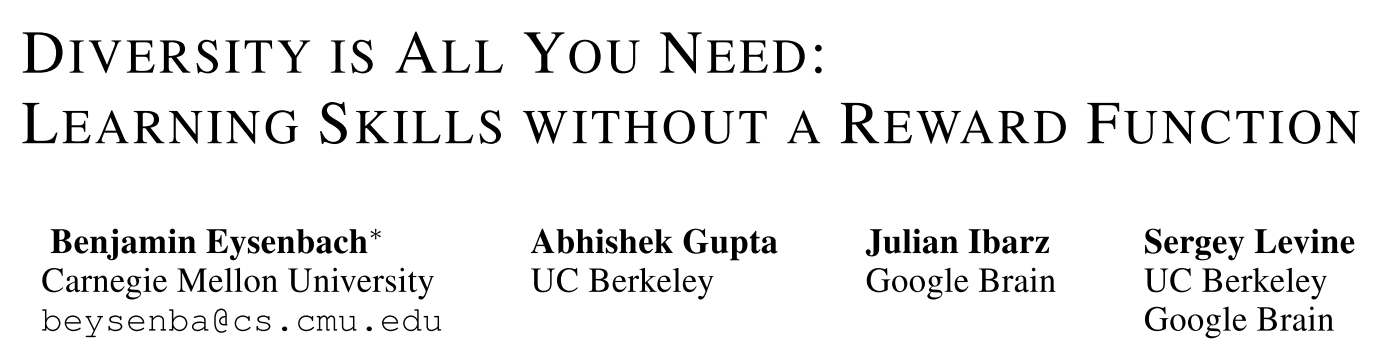
\includegraphics[width=0.8\textwidth]{imgs/DIAYN_tittle.png}
  \end{figure}
\end{frame}

\begin{frame}
  \frametitle{Motivation}
  \begin{itemize}
    \item Autonomous acquisition of useful skills without any reward signal.
    \item Why without any reward signal?
    \begin{itemize}
      \item for sparse rewards setting, learning useful skills without supervision may help address challenges in exploration
      \item serve as primitives for hierarchical RL, effectively shortening the episode length
      \item in many practical settings, interacting with the environment is essentially free, but evaluating the reward requires human feedback.
      \item it is challenging to design a reward function that elicits the desired behaviors from the agent(without imitation sample, hard to design a reward funciton)
      \item when given an unfamiliar environment, it is challenging to determine what tasks an agent should be able to learn
    \end{itemize}
  \end{itemize}
\end{frame}

\begin{frame}
  \frametitle{Motivation(cont.)}
  \begin{itemize}
    \item Autonomous acquisition of useful skills without any reward signal.
    \item How to define "useful skills"?
    \begin{itemize}
      \item consider the setting where the reward function is unknown, so we want to learn a set of skills by \textbf{maximizing the utility of this set}
    \end{itemize}
    \item How to maximize the utility of this set?
    \begin{itemize}
      \item each skill individually is distinct
      \item the skills collectively explore large parts of the state space
    \end{itemize}
    \end{itemize}
\end{frame}

\begin{frame}
  \frametitle{Key Idea: Using discriminability between skills as an objective}
  \begin{itemize}
    \item design a reward function which only depends on CMP
    \item skills are just distinguishable \xmark
    \item skills diverse in a semantically meaningful way \cmark
    \begin{itemize}
      \item action distributions \xmark (actions that do not affect the environment are not visible to an outside observer)
      \item state distributions \cmark
    \end{itemize}
  \end{itemize}
\end{frame}

\begin{frame}
  \frametitle{How It Works}
  \begin{itemize}
    \item [1] skill to dictate the states that the agent visits
    \begin{itemize}
      \item one-to-one correspondence between skill and Z(for any certain time, parameters $\theta$ is fixed)
      \item $Z \sim p(z)$, which means Z is different with each other
      \item make state distributions depend on Z(vice versa.), then state distributions become diverse
    \end{itemize}
    \item [2] ensure that states, not actions, are used to distinguish skills
    \begin{itemize}
      \item given state, action is not related to skill
      \item make action directly depends on skill is a \textbf{trivial} method, we better avoid it
    \end{itemize}
    \item [3] viewing all skills together with p(z) as a mixture of policies, we maximize the entropy $\mathcal{H}[A \mid S]$
    \item Attention: \textcolor{NJUPurple}{2} maybe causes the network don't care input Z, but \textcolor{NJUPurple}{1} avoids it; maybe causes output(action) become same one, but \textcolor{NJUPurple}{3} avoids it
  \end{itemize}

  $$
  \begin{aligned}
  \mathcal{F}(\theta) & \textcolor{red}{\triangleq I(S ; Z)+\mathcal{H}[A \mid S]-I(A ; Z \mid S)} \\
  &=(\mathcal{H}[Z]-\mathcal{H}[Z \mid S])+\mathcal{H}[A \mid S]-(\mathcal{H}[A \mid S]-\mathcal{H}[A \mid S, Z]) \\
  &=\mathcal{H}[Z]-\mathcal{H}[Z \mid S]+\mathcal{H}[A \mid S, Z]
  \end{aligned}
  $$
\end{frame}


\begin{frame}
  \frametitle{How It Works(cont.)}
  $$
  \begin{aligned}
  \mathcal{F}(\theta) & \triangleq I(S ; Z)+\mathcal{H}[A \mid S]-I(A ; Z \mid S) \\
  &=(\mathcal{H}[Z]-\mathcal{H}[Z \mid S])+\mathcal{H}[A \mid S]-(\mathcal{H}[A \mid S]-\mathcal{H}[A \mid S, Z]) \\
  &=\textcolor{red}{\mathcal{H}[Z]-\mathcal{H}[Z \mid S]+\mathcal{H}[A \mid S, Z]}
  \end{aligned}
  $$
  \begin{itemize}
    \item [1] fix p(z) to be uniform in our approach, guaranteeing that is has maximum entropy
    \item [2] it should be easy to infer the skill z from the current state
    \item [3] each skill should act as randomly as possible
  \end{itemize}
\end{frame}

\begin{frame}
  \frametitle{How It Works(cont.)}
  $$
  \begin{aligned}
    \mathcal{F}(\theta) &=\mathcal{H}[A \mid S, Z]-\mathcal{H}[Z \mid S]+\mathcal{H}[Z] \\
    &=\mathcal{H}[A \mid S, Z]+\mathbb{E}_{z \sim p(z), s \sim \pi(z)}[\log p(z \mid s)]-\mathbb{E}_{z \sim p(z)}[\log p(z)] \\
    & \geq \mathcal{H}[A \mid S, Z]+\mathbb{E}_{z \sim p(z), s \sim \pi(z)}\left[\log q_{\phi}(z \mid s)-\log p(z)\right] \triangleq \mathcal{G}(\theta, \phi)
  \end{aligned}
  $$
  \begin{itemize}
    \item $\mathcal{G}(\theta, \phi)$ is a variational lower bound
  \end{itemize}
\end{frame}

\begin{frame}
  \frametitle{Implementation}
  \begin{minipage}{0.45\linewidth}
    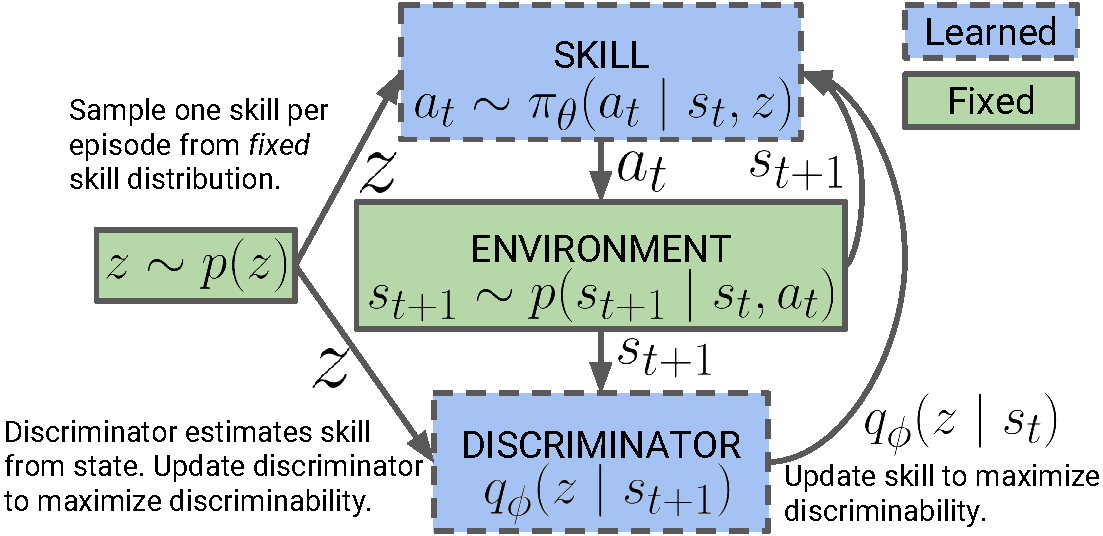
\includegraphics[width=\linewidth]{imgs/model.pdf}
  \end{minipage} \hfill
  \begin{minipage}{0.45\linewidth}
    \begin{itemize}
      \item maxize a cumulative pseudo-reward by SAC
      \item pseudo-reward: $r_{z}(s, a) \triangleq \log q_{\phi}(z \mid s)-\log p(z)$
    \end{itemize}
  \end{minipage}
\end{frame}

\begin{frame}
  \frametitle{Algorithm}
  \begin{algorithm}[H]
    \small
    \DontPrintSemicolon
    \SetAlgoLined
    \While{not converged}{
        Sample skill $z \sim p(z)$ and initial state $s_0 \sim p_0(s)$\;
        \For{$t \leftarrow 1$ \KwTo $steps\_per\_episode$}{
            Sample action $a_t \sim \pi_{\theta}(a_t \mid s_t, z)$ from skill.\;
            Step environment: $s_{t+1} \sim p(s_{t+1} \mid s_t, a_t)$.\;
            Compute $q_{\phi}(z \mid s_{t+1})$ with discriminator.\;
            Set skill reward $r_t = \log q_{\phi}(z \mid s_{t+1}) - \log p(z)$\;
            Update policy ($\theta$) to maximize $r_t$ with SAC.\;
            Update discriminator ($\phi$) with SGD.\;
        }
    } 
    \caption{DIAYN}
  \end{algorithm}
\end{frame}

\begin{frame}
  \frametitle{Applications}
  \begin{itemize}
    \item adapting skills to maximize a reward
    \item hierarchical RL
    \item imitation learning
    \item \textbf{unsupervised meta RL}
  \end{itemize}
\end{frame}

\section{Unsupervised Meta-Learning for Reinforcement Learning}
\begin{frame}
  \frametitle{Unsupervised Meta-Learning for Reinforcement Learnin}
  \begin{figure}
    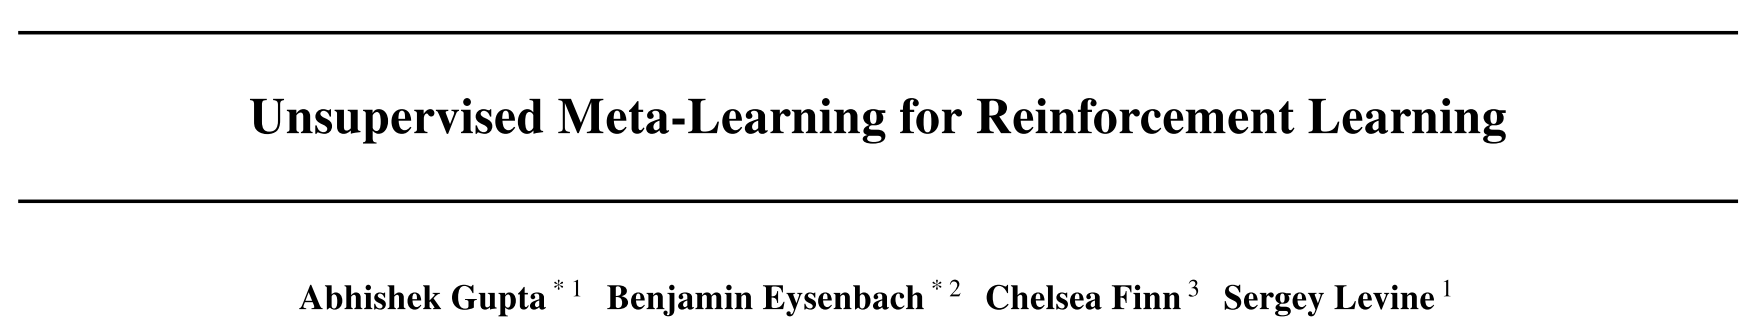
\includegraphics[width=0.8\textwidth]{imgs/UML_tittle.png}
  \end{figure}
\end{frame}


\begin{frame}
  \frametitle{Motivation}
  \begin{itemize}
    \item aim to do so without depending on any human supervision or information about the tasks that will be provided for meta-testing
    \item assumptions of prior work \xmark
    \begin{itemize}
      \item a fixed tasks distribution
      \item tasks of meta-train and meta-test are sample from this distribution
    \end{itemize}
    \item Why not pre-specified task distribution?
    \begin{itemize}
      \item specifying a task distribution is tedious and requires a significant amount of supervision
      \item the performance of meta-learning algorithms critically depends on the meta-training task distribution, and meta-learning algorithms generalize best to new tasks which are drawn from the same distribution as the meta-training tasks
    \end{itemize}
    \item assumptions of this work: the environment dynamics(CMP) remain the same
    \item \textbf{"environment-specific learning procedure"}
  \end{itemize}
\end{frame}

\begin{frame}
  \frametitle{Attention}
  \begin{itemize}
    \item this paper have been rejected(maybe twice)
    \item this paper make some vary strong assumption when analysising:
    \begin{itemize}
      \item deterministic dynamics(the "future work" of 2018, but authors maybe forget it...)
      \item only get a reward when the end state(two case have been concerned)
    \end{itemize}
    \item the expriment may be not enough and convincing
    \item there are something wrong (at least ambiguous) in the paper...
  \end{itemize}
\end{frame}


\begin{frame}
  \frametitle{Definition of Terminology and Symbol}
  \begin{itemize}
    \item MDP: $M=(S, A, P, \gamma, \rho, r)$
    \item CMP: $C=(S, A, P, \gamma, \rho)$
    \item S: state space 
    \item A: action space 
    \item P: transition dynamics 
    \item $\gamma$: discount factor
    \item $\rho$: initial state distribution 
    \item dataset of experience(for MDP): $\mathcal{D}=\left\{\left(s_{i}, a_{i}, r_{i}, s_{i}^{\prime}\right)\right\} \sim M$
    \item learning algorithm(for MDP): $f: \mathcal{D} \rightarrow \pi$
  \end{itemize}
\end{frame}

\begin{frame}
  \frametitle{Definition of Terminology and Symbol(cont.)}
  \begin{itemize}
    \item for CMP: $R(f, r_z) = \sum_i \E_{\substack{\pi = f(\{\tau_1, \cdots, \tau_{i-1}\}) \\ \tau \sim \pi}} \left[\sum_t r_z(s_t, a_t) \right]$
    \item evaluate the learning procedure f by summing its cumulative reward across iterations
  \end{itemize}
\end{frame}

\begin{frame}
  \frametitle{Key Idea}
  \begin{itemize}
    \item from the perspective of "no free lunch theorem": 
    
    the assumption that the dynamics remain the same across tasks affords us an inductive bias with which we pay for our lunch
    \item our results are lower bounds for the performance of general learning procedures
  \end{itemize}
\end{frame}

\begin{frame}
  \frametitle{Regret for certain Task Distribution(given CMP)}
  \begin{itemize}
    \item For a task distribution $p(r_z)$, the optimal learning procedure $f^∗$ is given by\\
    $f^{*} \triangleq \arg \max _{f} \mathbb{E}_{p\left(r_{z}\right)}\left[R\left(f, r_{z}\right)\right]$
    \item regret of a certain learning procedure and task distribution:\\
    $\operatorname{REGRET}\left(f, p\left(r_{z}\right)\right) \triangleq \mathbb{E}_{p\left(r_{z}\right)}\left[R\left(f^{*}, r_{z}\right)\right]-\mathbb{E}_{p\left(r_{z}\right)}\left[R\left(f, r_{z}\right)\right]$
    \item Obviously\\$f^{*} \triangleq \arg \min _{f} \operatorname{REGRET}\left(f, p\left(r_{z}\right)\right) $\\
    and\\$\operatorname{REGRET}\left(f^*, p\left(r_{z}\right)\right)  = 0$
    \item $f^*$ should be the output of traditional "meta RL algorithm"
  \end{itemize}
\end{frame}

\begin{frame}
  \frametitle{Regret for worst-case Task Distribution(given CMP)}
  \begin{itemize}
    \item evaluate a learning procedure $f$ based on its regret against the worst-case task distribution for CMP $C$:\\
    $\operatorname{REGRET}_{\mathrm{WC}}(f, C)=\max _{p\left(r_{z}\right)} \operatorname{REGRET}\left(f, p\left(r_{z}\right)\right)$
    \item by this way, we do not need any prior knowledge of $p(r_z)$
    \item Attention: CMP may lead to \textbf{inductive bias}
  \end{itemize}
\end{frame}

\begin{frame}
  \frametitle{Optimal Unsupervised Learning Procedure}

  \begin{definition}
    The optimal unsupervised learning procedure $f_C^*$ for a CMP $C$ is defined as
    \begin{equation*}
    \vspace{-1em}
        f_C^* \triangleq \argmin_f \textsc{Regret}_{\textsc{WC}}(f, C).
    \end{equation*}
    \end{definition}
    \begin{itemize}
      \item "unsupervised" means you do not need "reward"(like DIAYN)
      \item $f_C^*$ should be the output of our "unsupervised meta RL algorithm"
    \end{itemize}
\end{frame}

\begin{frame}
  \frametitle{Optimal Unsupervised Meta-learner}

   \begin{definition}
  The optimal unsupervised meta-learner $\gF^*(C) = f_C^*$ is a function that takes as input a CMP $C$ and outputs the corresponding optimal unsupervised learning procedure $f_C^*$:
  \begin{equation*}
  \vspace{-1em}
      \gF^* \triangleq \argmin_{\gF} \textsc{Regret}_{\textsc{WC}}(\gF(C), C)
  \end{equation*}
  \end{definition}
  
  \begin{itemize}
    \item the optimal unsupervised meta-learner $\gF^*$ is universal, it does not depend on any particular task distribution, or any particular CMP
  \end{itemize}
\end{frame}

\begin{frame}
  \frametitle{Min-Max}
  \begin{figure}
  \centering
  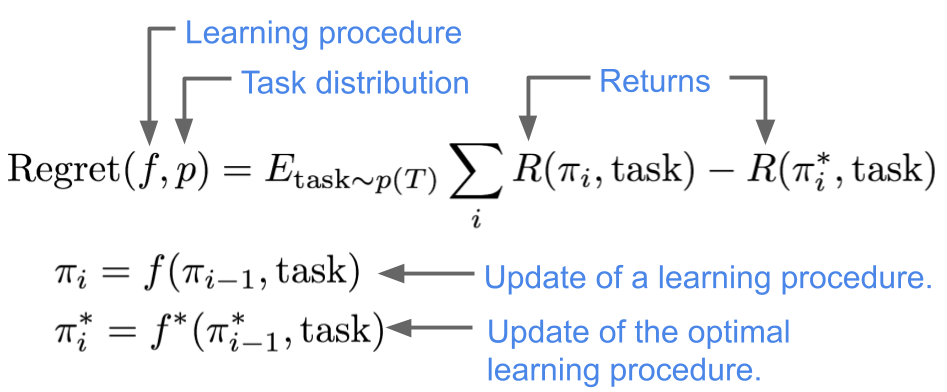
\includegraphics[width=0.7\linewidth]{imgs/labeled_regret_v2.png}
  \end{figure}

  $$\min _{f} \max _{p} \quad \operatorname{Regret}(f, p)$$
\end{frame}

\begin{frame}
  \frametitle{Analysis by Case Study}
  \begin{itemize}
    \item Special Case: Goal-Reaching Tasks
    \item General Case: Trajectory-Matching Tasks
    \item in these case, we make some assumption such as deterministic dynamics, then generalize it
  \end{itemize}
  

\end{frame}

\begin{frame}
  \frametitle{Special Case: Goal-Reaching Tasks}

  consider episodes with finite horizon T and a discount factor of $\gamma = 1$\\
  reward: $r_{g}\left(s_{t}\right) \triangleq \mathbf{1}(t=T) \cdot \mathbf{1}\left(s_{t}=g\right)$
  \begin{figure}
    \centering
    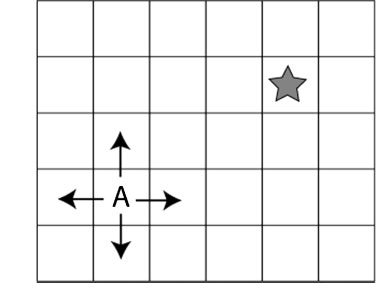
\includegraphics[width=0.4\linewidth]{imgs/Grid-world-problem-The-agent-moves-in-four-directions-to-find-the-goal-marked-with-a.png}
    \end{figure}
\end{frame}

\begin{frame}
  \frametitle{Optimal Learing Procedure for known $p(s_g)$}
  \begin{itemize}
    \item Define $f_\pi$ as the learning procedure that \textbf{uses policy $\pi$ to explore until the goal is found}, and then always returns to the goal state($f$ is a learning procedure, which is something like SAC or PPO...)
    \item the goal of meta-RL (for known $p(s_g)$): find the best exploration policy $\pi$
    \item probability that policy $\pi$ visits state $s$ at time step $t = T$: $\rho_{\pi}^{T}(s)$
    \item expected hitting time of this goal state: \\
    $$\mathrm{HITTINGTIME}_{\pi}\left(s_{g}\right)=\frac{1}{\rho_{\pi}^{T}\left(s_{g}\right)}$$
    \item tips: "hitting time" means the \textbf{epected number of episodes} we need to make our end-state to be the goal-state(explore by the given policy $\pi$)
    \end{itemize}
\end{frame}

\begin{frame}
  \frametitle{Optimal Learing Procedure for known $p(s_g)$(cont.)}
  \begin{itemize}
    \item difinition of regret: \\
    $$\operatorname{REGRET}\left(f, p\left(r_{z}\right)\right) \triangleq \mathbb{E}_{p\left(r_{z}\right)}\left[R\left(f^{*}, r_{z}\right)\right]-\mathbb{E}_{p\left(r_{z}\right)}\left[R\left(f, r_{z}\right)\right]$$
    \item regret of the learning procedure $f_\pi$:\\
    $$\operatorname{REGRET}\left(f_{\pi}, p\left(r_{g}\right)\right)=\int\mathrm{HITTINGTIME}_{\pi}\left(s_{g}\right) p\left(s_{g}\right) d s_{g}=\int \frac{p\left(s_{g}\right)}{\rho_{\pi}^{T}\left(s_{g}\right)} d s_{g}$$
    \item exploration policy for the optimal meta-learner, $\pi^*$, satisfies: \\
    $$\rho_{\pi^{*}}^{T}\left(s_{g}\right)=\frac{\sqrt{p\left(s_{g}\right)}}{\int \sqrt{p\left(s_{g}^{\prime}\right)} d s_{g}^{\prime}}$$
  \end{itemize}
\end{frame}

\begin{frame}
  \frametitle{Optimal Learing Procedure for Unknown $p(s_g)$}
  \begin{lemma} \label{lemma:uniform}
    Let $\pi$ be a policy for which $\rho_\pi^T(s)$ is uniform. Then $f_\pi$ is has lowest worst-case regret among learning procedures in $\gF_\pi$.
  \end{lemma}
  (proof is straight by disproval)

  \begin{itemize}
    \item finding such a policy $\pi$ is challenging, especially in \textbf{high-dimensional} state spaces and in the absense of resets
    \item acquiring $f_\pi$ directly without every computing $\pi$
  \end{itemize}
\end{frame}

\begin{frame}
  \frametitle{Optimal Learing Procedure for Unknown $p(s_g)$(cont.)}
  \begin{itemize}
    \item what we want: $\rho_\pi^T(s)$ is a uniform distribution
    \item how to do: define a latent variable $z$, make $z$ and $s_T$, and sample $z$ from a uniform distributions
    \item there exists a conditional distribution $\mu(s_T | z)$ (more detail later), change it to maximize the mutual information:\\
    $$\max _{\mu\left(s_{T} \mid z\right)} I_{\mu}\left(s_{T} ; z\right)$$
    \item still need to make sure maximize the mutual information can make $s_T$ uniform
  \end{itemize}
\end{frame}

\begin{frame}
  \frametitle{Optimal Learing Procedure for Unknown $p(s_g)$(cont.)}
  \begin{lemma} \label{lemma:MImax}
    Assume there exists a conditional distribution $\mu(s_T \mid z)$ satisfying the following two properties:
    \begin{enumerate}
        \item The marginal distribution over terminal states is uniform: $\mu(s_T) = \int \mu(s_T \mid z) \mu(z) dz = \textsc{Unif}(\gS)$; and
        \item The conditional distribution $\mu(s_T \mid z)$ is a Dirac: $\forall z, s_T \; \exists s_z \text{ s.t. } \mu(s_T \mid z) = \mathbf{1}(s_T = s_z)$.
    \end{enumerate}
    Then any solution $\mu(s_T \mid z)$ to the mutual information objective satisfies the following:
    % distribution $\mu^* \in \gP_\mu$ such that $\mu^*(s_T) = \textsc{Unif}(\gS)$ is uniform over goal states and $\mu^*(s_T \mid z) \stackrel{d}{=} \mathbbm{1}(s_T = s_z)$ is a Dirac distribution, centered at a state $s_z$ specified by the latent $z$. Then any distribution $\mu$ that maximizes mutual information $I_\mu(s_T; z)$ satisfies 
    \begin{equation*}
    \mu(s_T) = \textsc{Unif}(\gS) \quad \text{and} \quad \mu(s_T \mid z) = \mathbf{1}(s_T = s_z).
    \end{equation*}
    \end{lemma}
\end{frame}

\begin{frame}
  \frametitle{Optimal Learing Procedure for Unknown $p(s_g)$(cont.)}
  \begin{itemize}
    \item how to get $\mu(s_T | z)$ ?
    \item define a latent-conditioned policy $\mu(a \mid s,z)$
    \item then we have\\ $$\mu(\tau, z)=\mu(z) p\left(s_{1}\right) \prod_{t} p\left(s_{t+1} \mid s_{t}, a_{t}\right) \mu\left(a_{t} \mid s_{t}, z\right)$$
    \item get marginal likelihood by integrate the trajectory except $s_T$\\$$\mu\left(s_{T}, z\right)=\int \mu(\tau, z) d s_{1} a_{1} \cdots a_{T-1}$$
    \item divide by $\mu(z)$ (which is a uniform distribution): $\mu(s_T\mid z) = \frac{\mu\left(s_{T}, z\right)}{\mu(z)}$
    \item then make $r_{z}\left(s_{T}, a_{T}\right) \triangleq \log p\left(s_{T} \mid z\right)$
  \end{itemize}
\end{frame}

\begin{frame}
  \frametitle{Optimal Learing Procedure for Unknown $p(s_g)$(cont.)}
  what wrong with it?
  \begin{equation*}
    \begin{aligned}
      I_\mu(s_T;z)&=\mathcal{H}[S_T] - \mathcal{H}[S_T\mid Z]\\
      &=\mathbb{E}_{z \sim p(z), s_T \sim \mu(s_T\mid z)}[\log \mu(s_T \mid z) - \log \mu(s_T)]
    \end{aligned}
  \end{equation*}
  but... how to get $\log \mu(s_T)$?
  \begin{equation*}
    \begin{aligned}
      I_\mu(s_T;z)&=\mathcal{H}[Z] - \mathcal{H}[Z\mid S_T]\\
      &=\mathbb{E}_{z \sim p(z), s_T \sim \mu(s_T\mid z)}[\log \mu(z\mid s_T) - \log \mu(z)]
    \end{aligned}
  \end{equation*}
  $\log \mu(z\mid s_T)$ is also difficult to get(because we do not have $\mu(s_T)$), but we can learn $\mu(z\mid s_T)$ directedly, just like DIAYN
\end{frame}

\begin{frame}
  \frametitle{General Case: Trajectory-Matching Tasks}
  \begin{itemize}
    \item “trajectory-matching” tasks: only provide a positive reward when the policy executes the \textbf{optimal trajectory}\\$$r_{\tau}^{*}(\tau) \triangleq \mathbf{1}\left(\tau=\tau^{*}\right)$$
    \item trajectory-matching case is actually a generalization of the typical reinforcement learning case with Markovian rewards
    \item hitting time and regret (for known $p(\tau^*)$)\\
    $$\mathrm{HITTINGTIME}_{\pi}\left(\tau^{*}\right)=\frac{1}{\pi\left(\tau^{*}\right)}$$
    $\operatorname{REGRET}\left(f_{\pi}, p\left(r_{\tau}\right)\right)=\int \left.\mathrm{HITTING} \operatorname{TIME}_{\pi}(\tau) p(\tau) d \tau\right)=\int \frac{p(\tau)}{\pi(\tau)} d \tau$
  \end{itemize}
\end{frame}

\begin{frame}
  \frametitle{General Case: Trajectory-Matching Tasks(cont.)}
  for unknow $p(\tau^*)$, we have lemma, again
  \begin{lemma}
    Let $\pi$ be a policy for which $\pi(\tau)$ is uniform. Then $f_\pi$ has lowest worst-case regret among learning procedures in $\gF_\pi$.
    \end{lemma}
    and we maxize the object just the same as last time$$I(\tau ; z)=\mathcal{H}[\tau]-\mathcal{H}[\tau \mid z]$$
\end{frame}

\begin{frame}
  \frametitle{General Reward Maximizing Tasks}
  \begin{itemize}
    \item that trajectory-matching is a super-set of the problem of optimizing any possible Markovian reward function at test-time
    \item bounding the worst-case regret on $R_\pi$ minimizes an upper bound on the worst-case regret on $R_{s,a}$: $$\min _{r_{\tau} \in R_{\tau}} \mathbb{E}_{\pi}\left[r_{\tau}(\tau)\right] \leq \min _{r \in R_{s, a}} \mathbb{E}_{\pi}\left[\sum_{t} r\left(s_{t}, a_{t}\right)\right]$$
    \item (bound is too loose, is it realy work?)
  \end{itemize}
\end{frame}

\begin{frame}
  \frametitle{Algorithm}
  \begin{figure}
    \centering
    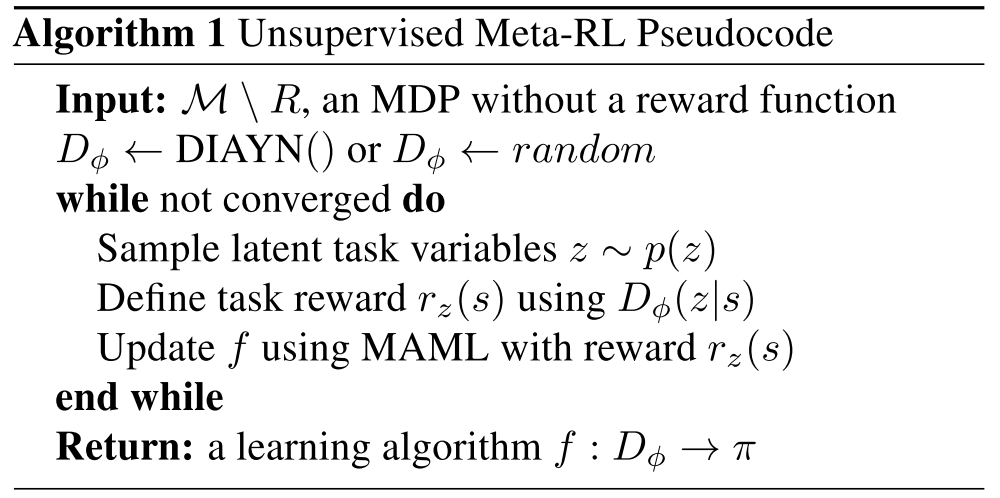
\includegraphics[width=0.8\textwidth]{imgs/agorithm.png}
  \end{figure}
\end{frame}

\begin{frame}
  \frametitle{Performance}
  Unsupervised meta-learning accelerates learning
  \begin{figure}
    \centering
    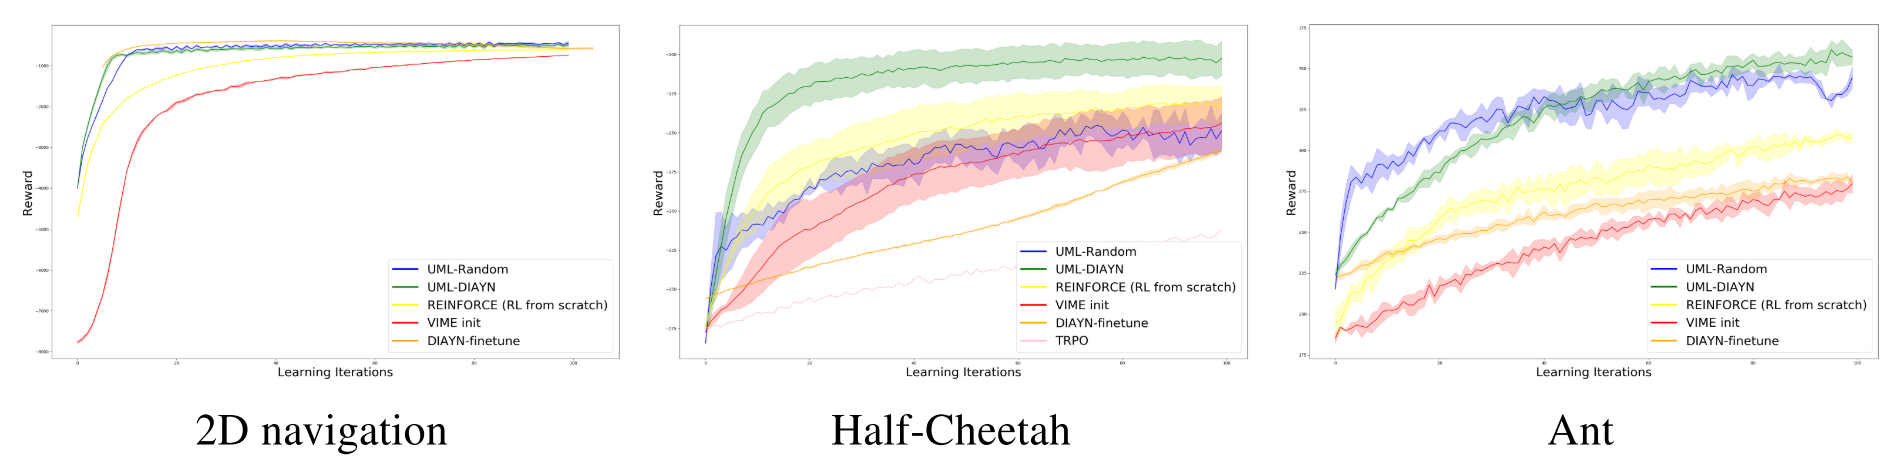
\includegraphics[width=0.8\textwidth]{imgs/performance1.png}
  \end{figure}
\end{frame}


  \begin{frame}
    \frametitle{Performance(cont.)}
    Comparison with handcrafted tasks
    \begin{figure}
      \centering
      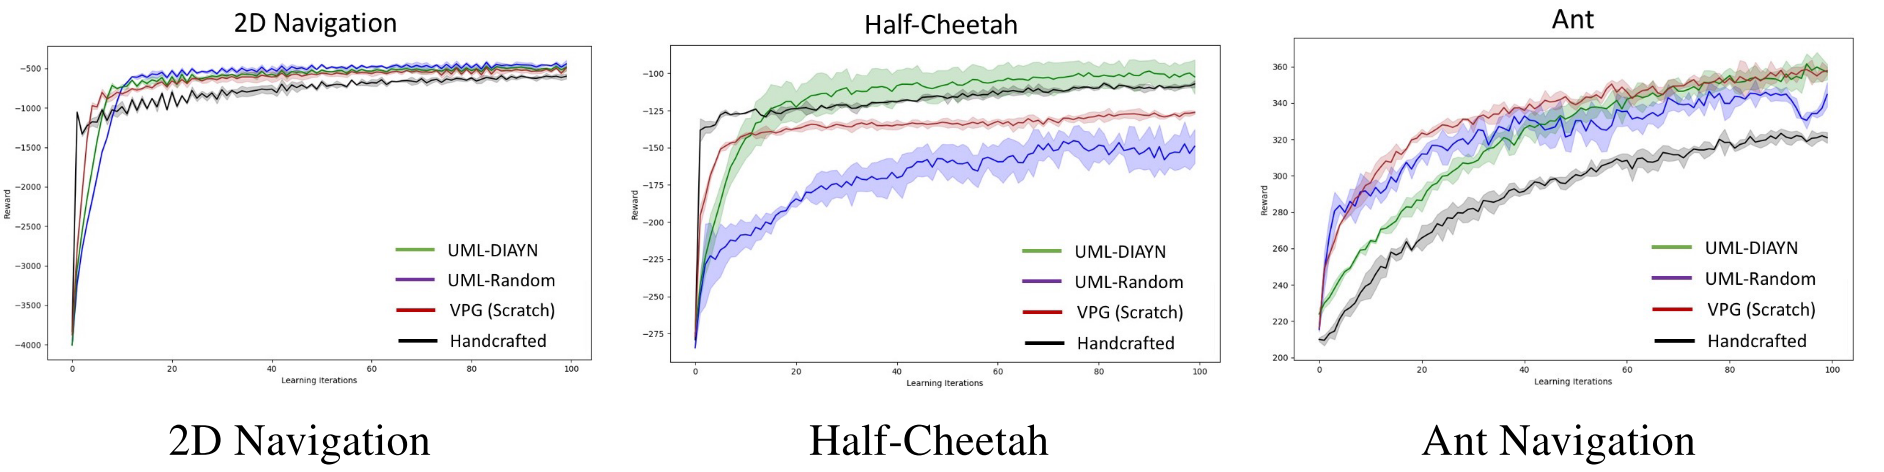
\includegraphics[width=0.8\textwidth]{imgs/performance2.png}
    \end{figure}
\end{frame}

\begin{frame}
  \frametitle{Discussion: 能不能再“无监督”一点?}
  \begin{itemize}
    \item 文中强调了他们的算法是基于给定CMP的情况下的,也就是说算法对reward mechanism不作要求,但是要求所有的task都有相同的CMP。
    \item 能否直接去掉“固定CMP”的约束?\xmark
    \item 能否使用其他meta-RL的方法,例如PEARL,得到关于CMP的context,再根据这个context做unsupervised meta-RL?
  \end{itemize}
\end{frame}

\begin{frame}
  \frametitle{Discussion: 能不能再“有监督”一点?}
  \begin{itemize}
    \item 文中一直再强调task distribution设计很困难,试图直接放弃设计task distribution,直接从CMP中获得prori knowledge。但是这样的方式完全抛弃了加入expert knowledge的可能性。
    \item 有没有更好的融合expert knowledge和environment dynamics的方式?
    \item 在Goal-Reaching Tasks中,如果到达goal state的奖赏不同,满足min-max的探索策略则将不再是均匀分布,而是和最终的奖赏有关。
  \end{itemize}
\end{frame}

\begin{frame}
  \frametitle{Discussion: 结合上面两点,能不能显式的使用对抗策略,在无监督meta-RL和监督meta-RL中寻找平衡?}
  \begin{itemize}
    \item 可以理解为,无监督meta-RL的精髓就是在给定某个特性(文中是CMP)后,根据对抗的思想得到一个“能在最差的情况下都表现的足够好的learning procedure”
    \item 文章中经过分析认为对抗的思想蕴含在“每个状态出现的频率相同”这一假设上。
    \item 是否可以结合前面的讨论,显式的对抗,使用更弱一点的假设,从而引入expert knowledge。
  \end{itemize}
\end{frame}

\begin{frame}
  \frametitle{Discussion: 关于stochastic dynamics}
  \begin{itemize}
    \item 被作者遗忘的"future work"
    \item 同样使用context-based表示dynamics
    \item 其实现在的方法可以直接应用在stochastic dynamics,但是需要更多的理论证明
  \end{itemize}
\end{frame}

\begin{frame}

\centering
\textbf{Thank You!}

\end{frame}
\end{document}